\chapter{算法设计和优化}

\section{InSAR 成像算法简介}

\subsection{InSAR 测高原理}

讨论并行 InSAR 数据处理算法前,先对 InSAR 成像原理做一个简单介绍。\cite{simons2007interferometric}

\begin{figure}[ht]
\centering
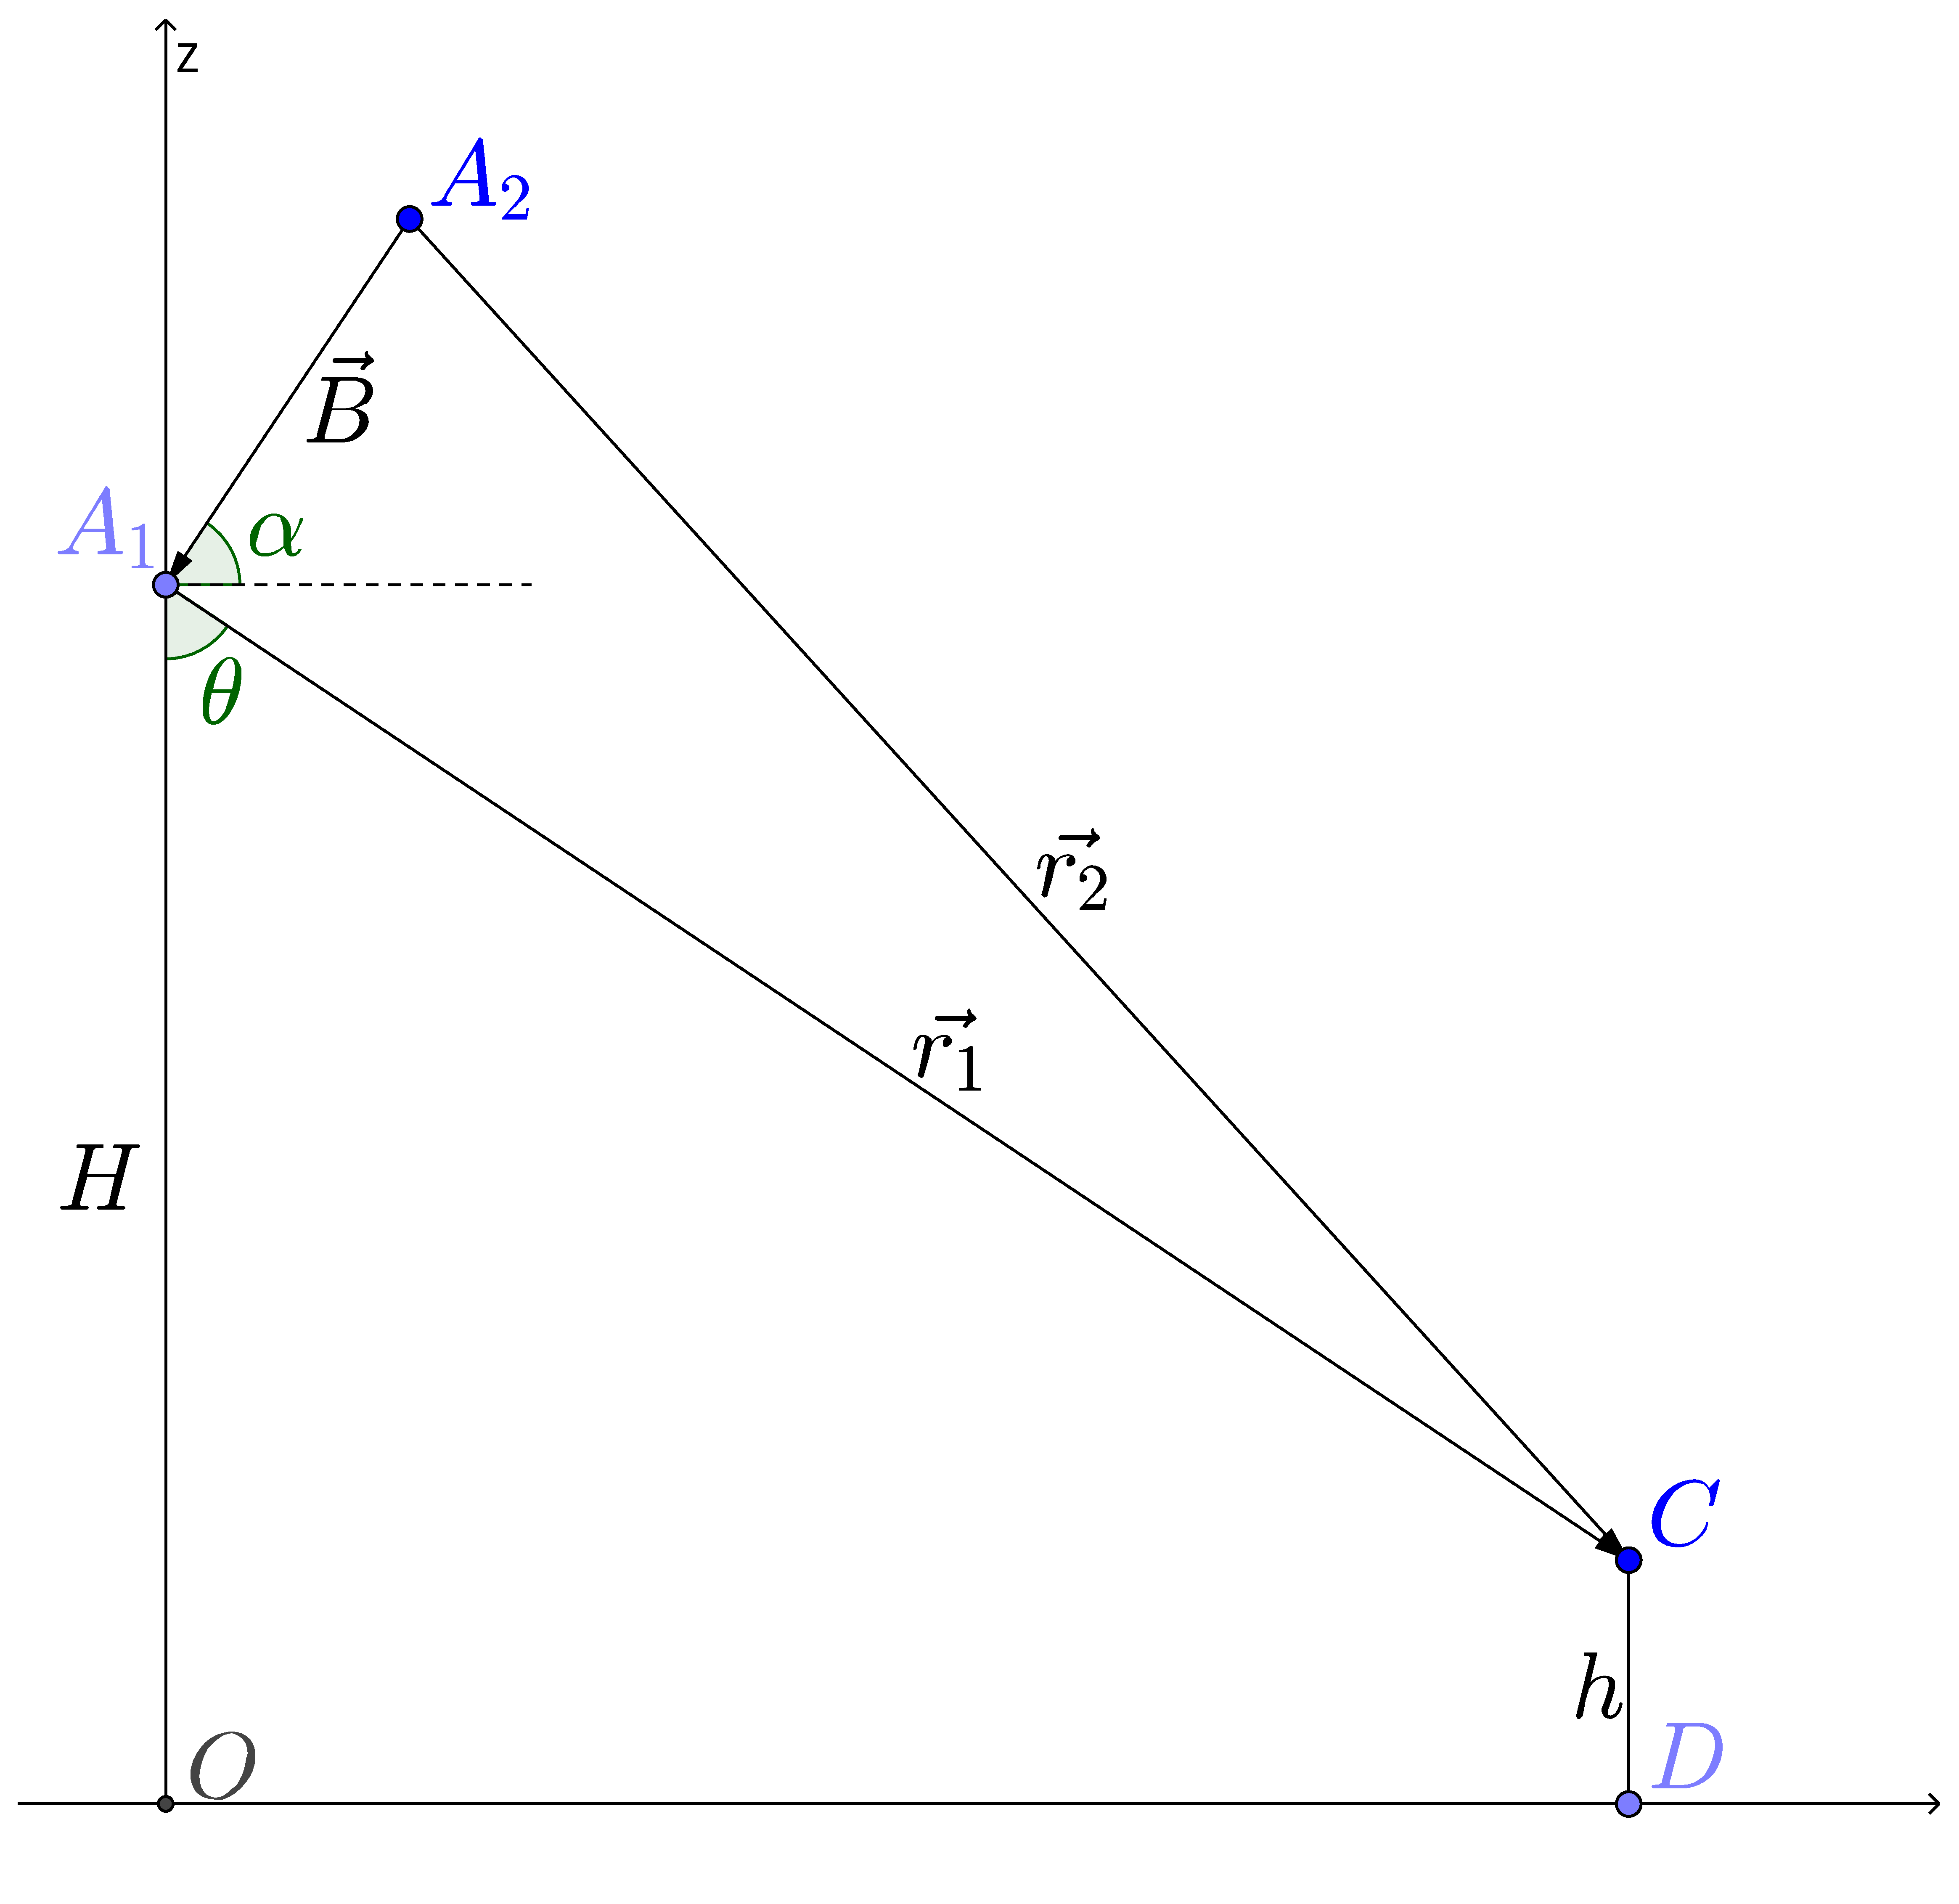
\includegraphics[width=0.4\textwidth]{insar_simple}
\caption{InSAR 高程测量基本原理} \label{fig:insar_simple}
\end{figure}

图 \ref{fig:insar_simple} 展示了利用两个 SAR 雷达观测同一地面单位进行 InSAR 测高的基本原理。InSAR 测量地表形变的原理与之类似。$A_1$ 和 $A_2$ 表示主天线和副天线位置,两天线空间位移矢量为 $\vec{B}$,称为 InSAR 基线,角度 $\alpha$ 为基线与水平面夹角。$C$ 为地面目标点,相对于两天线的位移矢量分别为 $\vec{r_1}$ 和 $\vec{r_2}$,称为斜距。角度 $\theta$ 为主天线观察方向与竖直方向的夹角,称为下视角。

斜距矢量 $ \vec{r_1} $ 和 $ \vec{r_2} $ 可以根据天线方向和微波信号双程旅行时得到;雷达位置或 SAR 卫星轨道,即基线 $\vec{B}$ 和天线高度 $H$,也可以认为是已知的。

由简单的几何关系可知,目标点高度可以表示为:

\begin{equation}
    h = H - r_1 \cos\theta
\end{equation}

为了得到 $\theta$,分别从主天线和副天线取得对焦后的 SAR 图像。该图像具有复数像素值,包含回波的幅度和相位信息(或目标点的散射系数),因此称为单视复数图像(Single Look Complex,SLC)。SLC 图像像素基本对应于 SAR 雷达最小分辨区域(数十米量级\cite{sandwell2011gmtsar})。

目标点 $C$ 在主、副 SLC 图像上的复像素值 $P_1$ 和 $P_2$ 可以表示为:

\begin{equation}
\begin{split}
    P_1(\vec{r_1}) = A_1(\vec{r_1}) \exp(i \frac{4\pi}{\lambda} r_1) \\
    P_2(\vec{r_2}) = A_2(\vec{r_2}) \exp(i \frac{4\pi}{\lambda} r_2) \\
\end{split}
\end{equation}

将两幅 SLC 图像共轭相乘,即得到一幅干涉图像:

\begin{equation}
    P_{\textrm{int}} = P_1^* P_2 =  A_1 A_2 \exp(i \frac{4\pi}{\lambda}(r_2 - r_1))
\end{equation}

干涉图相位项中的 $ r_2 - r_1 $ 可以通过余弦定理展开:
\begin{equation}
\begin{split}
    r_2 - r_1 &= r_1 (\frac{r_2}{r_1} - 1) \\
              &= r_1 \sqrt{1- \frac{\vec{r_1} \cdot \vec{B}}{r_1} + (\frac{B}{r_1})^2}
\end{split}
\end{equation}

基线长度 $B$ 一般远小于斜距 $r_1$、$r_2$,上式可以简化为:
\begin{equation}
    r_2 - r_1 = - \vec{r_1} \cdot \vec{B} = - r_1 B \cos(\frac{\pi}{2} - \theta + \alpha)
\end{equation}

故 $\theta$ 可以通过干涉图相位求出,进而得到目标点高程 $h$。然而,实际上回波相位总是折叠到一个 $2\pi$ 周期内的,因此干涉图相位也折叠在一个 $2\pi$ 周期中,这称为相位缠绕(phase wrap)。连续的相位值仍可以通过一些相位解缠算法估计出来。

实际的 SAR 雷达工作高度 $H$ 可达数十到数百千米,如 ALOS 卫星工作轨道高度为 700km\cite{web:alos},因此必须考虑地球曲率的影响。研究地表形变或位移时,原始地形引起的相位差也要通过数字高程模型去除。此外,轨道偏移、电离层噪声、对流层噪声等因素也会影响 InSAR 成像的精度。

\subsection{InSAR 成像算法}

虽然 InSAR 测高原理非常简单,但实际的成像算法要复杂得多。主要可以归纳为以下若干步骤\cite{sandwell2011gmtsar}:

\textbf{SAR 成像和预处理}:相位差的测量精度决定了 InSAR 测高的精度。进行干涉的两幅 SAR SLC 图像必须对成像区域有较好的聚焦,并且具有合适的基线长度,需要在若干组 SAR 数据中进行\textbf{筛选}。为了提取成像区域的有效信息,往往需要对 SAR 数据进行\textbf{拼接}或\textbf{切割}。

\textbf{图像配准}(image registration):因天线视角、轨道偏移等因素,主、副 SLC 图像成像区域往往有一定差异。进行干涉成像之前,要通过图像配准将副 SLC 图像映射到和主 SLC 图像同样的成像区域。图像配准是 InSAR 数据处理中计算复杂度较高的一个步骤。

\textbf{干涉成像}:将对齐的主副 SAR SLC 图像进行共轭相乘,得到干涉图像。干涉图的相位信息反映了地面高程或地表位移信息,但被折叠到一个 $2\pi$ 周期上。

\textbf{相位修正}:根据研究对象的不同,从干涉图中可选地去除地形相位、电离层延迟等不需要的相位项,以及滤除各种影响结果精度的噪声。

\textbf{相位解缠}:利用高程或形变的连续性,从折叠相位恢复出连续变化的相位,以在较大的尺度上反映高程或形变信息。相位解缠是 InSAR 数据处理中技巧性比较高的一个步骤。

上述步骤即为 InSAR 成像程序的主要功能。除此之外,包括 GMTSAR 在内的 InSAR 处理软件还包含很多其他辅助分析模块,研究人员可以查阅相关文档以进一步了解。


\section{InSAR 成像算法 CPU 并行优化}

本节将以 GMTSAR 中图像拼接预处理和相位解缠两个程序模块为例子,介绍 CPU 并行的 InSAR 成像程序的算法设计和具体实现。

\subsection{并行图像配准算法}

InSAR 干涉成像要求输入的主、副 SAR SLC 图像精确对应同样的成像区域,以确保干涉图的相干性。但由于轨道偏移、天线视角、采样率变化(由天线移动速度差异或工作参数变化导致)等因素,副 SLC 图像成像区域相对主 SLC 图像成像区域会发生位移、旋转、拉伸等类型的畸变。图像配准的目的是找到主、副 SLC 图像坐标间的映射关系,以消除这些畸变。

在各类导致图像偏移的因素中,轨道偏移和雷达视角差异是主要的影响因素。这部分偏移可以通过精确的 SAR 天线轨道坐标与工作状态计算出。\citet{sandwell2011gmtsar} 指出,对于 ALOS 等星载 SAR 雷达,基于精确轨道数据计算的偏移量在方位向精度为大约2像素、距离向大约1像素。但 InSAR 成像往往要求达到至少 1/10 像素的配准精度 \cite{li2008image},因此除了利用已知的轨道参数进行\textbf{粗配准},还必须利用两幅图像本身的相关性进行\textbf{精配准}。

图像配准的精确性一般通过配准后图像的\textbf{相干性}(coherence)进行评估。对于两幅 SLC 图像 $P_1$ 和 $P_2$,在像素 $(x, y)$ 周围某个采样区域 $D(x, y)$ 上的相干性 $\gamma(x, y)$ 定义为:

\begin{equation}
    \gamma(x, y) = \frac{\sum_{x', y'} P_1(x', y') P_2^*(x', y')}{\sqrt{\sum_{x', y'}|P_1(x', y')|^2 \sum_{x', y'}|P_2(x', y')|^2}} \qquad (x', y') \in D(x, y)
    \label{eq:coherence}
\end{equation}

GMTSAR 中的 xcorr 和 fitoffset.csh 程序实现了图像配准,它将主 SAR SLC 图像像素到副 SLC 图像之间的映射近似为一个二维仿射变换。即副 SLC 图像上的坐标 $(x_i', y_i')$ 与主 SLC 图像坐标 $(x_i, y_i)$ 通过6个仿射变换参数相联系:

\begin{equation}
\begin{bmatrix}
  t_i x_i' \\
  t_i y_i' \\
  t_i \\
\end{bmatrix}
= \begin{bmatrix}
       a & b & c \\
       d & e & f \\
       0 & 0 & 1 \\
\end{bmatrix}
\begin{bmatrix}
  x \\
  y \\
  1 \\
\end{bmatrix}
\end{equation}

如图 \ref{fig:register} 所示,xcorr 从主 SLC 图像中等间隔选取 $n_x \times n_y $ 个大小为 $w_x \times w_y$ 的采样位置 $(x_c, y_c)_{i,j}$($0 \leq j < n_x$,$0 \leq i < n_y$)。一个采样位置映射到副 SLC 图像中的坐标 $(x'_c, y'_c)_{i,j}$ 可以看作在粗配准偏移矢量 $(\Delta_x, \Delta_y)$ 的基础上加上一个局部修正项 $(\delta_x, \delta_y)_{i,j}$,即:

\begin{equation}
    (x'_c, y'_c)_{i,j} = (x_c, y_c)_{i,j} + (\Delta_x, \Delta_y) + (\delta_x, \delta_y)_{i,j}
\end{equation}

\begin{figure}[htbp]
\centering
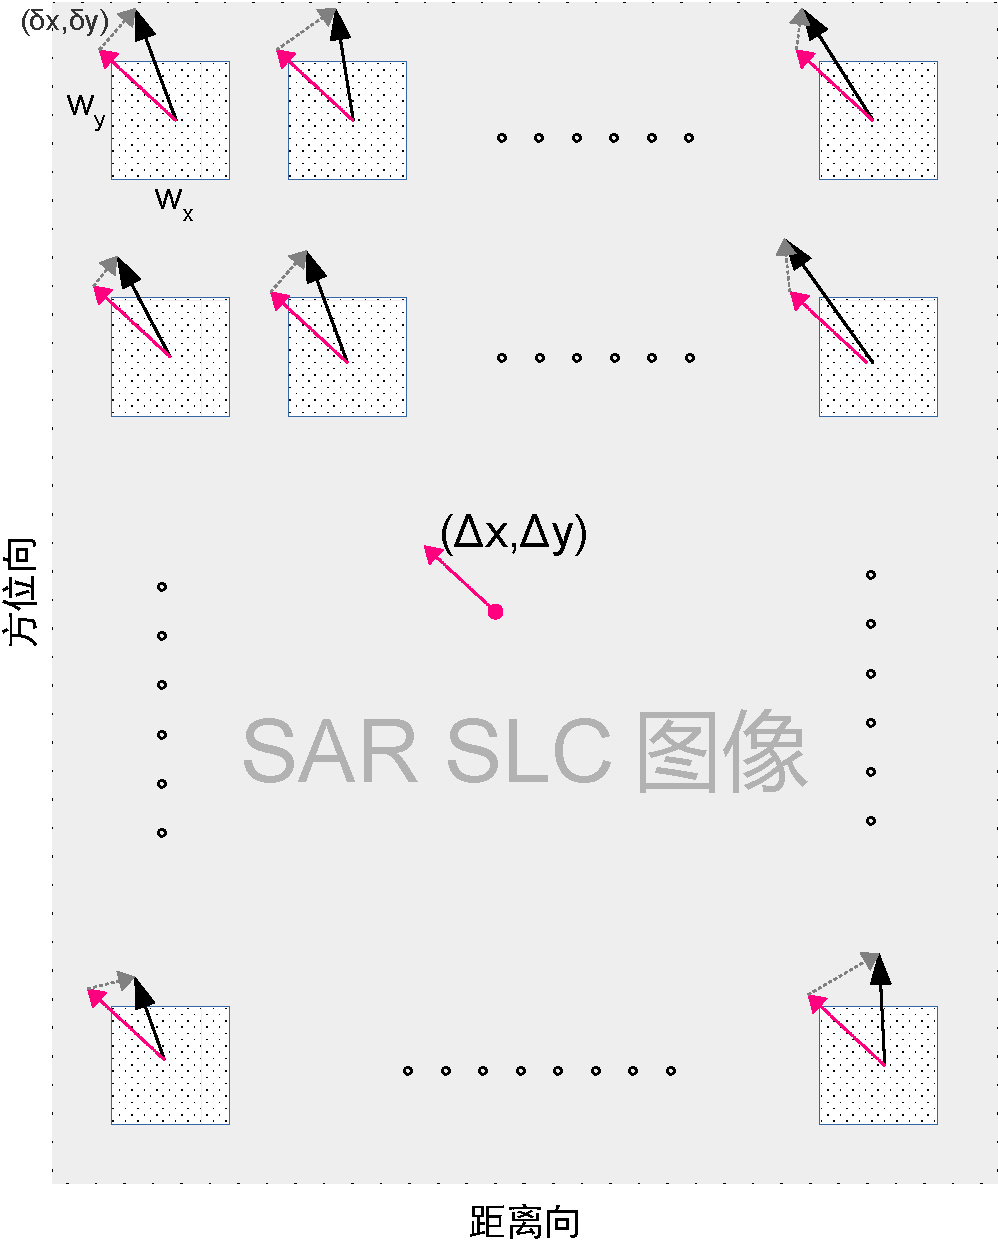
\includegraphics[width=0.6\textwidth]{register}
\caption{GMTSAR xcorr 配准算法示意} \label{fig:register}
\end{figure}

如前文所述,$\Delta_x$、$\Delta_y$ 已经可以提供几个像素的配准精度,因此可以在一个较小的采样窗口中搜索 $(\delta_x, \delta_y)$(xcorr 默认采样窗口大小 $w_x \times w_y = 64 \times 64$)。xcorr 通过局部搜索(散射系数幅度)的互相关最大值来判断修正项的大小。即,对于主 SLC 图像中以 $(x_c, y_c)$ 为中心的采样窗口 $D_1$ 和副 SLC 图像中以 $(x_c + \Delta_x, y_c + \Delta_y)$ 为中心的采样窗口 $D_2$,计算出互相关矩阵 $D_1 \star D_2$,局部的偏移矢量修正项 $(\delta_x, \delta_y)$ 满足:

\begin{equation}
    (D_1 \star D_2)[\delta_x, \delta_y] = \max(D_1 \star D_2)
\end{equation}

得到各个采样位置的精配准偏移量后,fitoffset.csh 选取其中互相关性较好的数据,通过最小二乘法拟合出6个仿射变换参数。

搜索互相关矩阵至多达到到1个像素的配准精度。为了得到次像素级精度的偏移矢量,需要对原始数据或互相关矩阵进行插值处理。目前并没有一个公认有效的插值方法,不同论文选择的插值算法、插值顺序都有所区别\cite{li2008image}\cite{hanssen1999evaluation}。对于每个采样窗口,xcorr 在计算互相关矩阵前后分别进行了两次 sinc 插值(具体算法流程如图 \ref{fig:xcorr} 所示):

\textbf{原始采样窗口像素的距离向插值}:如前文所述,粗配准精度在距离向上比方位向上更差一些。为了补偿这一精度差异,xcorr 计算互相关矩阵前在距离向对采样窗口像素进行 sinc 插值。sinc 插值可以通过 FFT 和频域补0高效地实现。插值因子默认 $\iota_r = 2$。

\textbf{互相关矩阵插值}:对互相关矩阵进行插值是获得次像素精度偏移矢量的常用方法,一般采用线性插值、sinc 插值或者样条插值方法。这一步 xcorr 使用的仍是 sinc 插值,插值在方位向和距离向都要进行,默认插值因子 $\iota_x = \iota_y = 16$。

图 \ref{fig:xcorr} 的局部配准算法仍有改进空间。前述图像配准算法只用到 SLC 图像幅度信息。除了距离向插值要使用复序列 FFT 对原始序列进行处理,后面的算法流程实际上已经抛弃了相位信息,因此可以使用实序列 FFT 算法(FFT of real data,RFFT)处理采样窗口和互相关矩阵即可。处理实序列时,RFFT 比复序列 FFT 节省一半的运行时间和存储空间。改进后的局部配准流程如图 \ref{fig:xcorr2} 所示。

\begin{figure}[htbp]
\centering
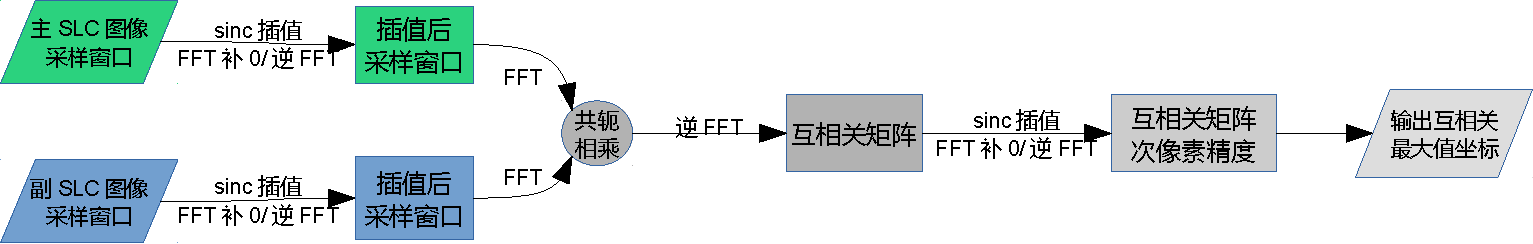
\includegraphics[width=0.99\textwidth]{xcorr-crop}
\caption{GMTSAR xcorr 局部配准算法流程} \label{fig:xcorr}
\end{figure}

\begin{figure}[htbp]
\centering
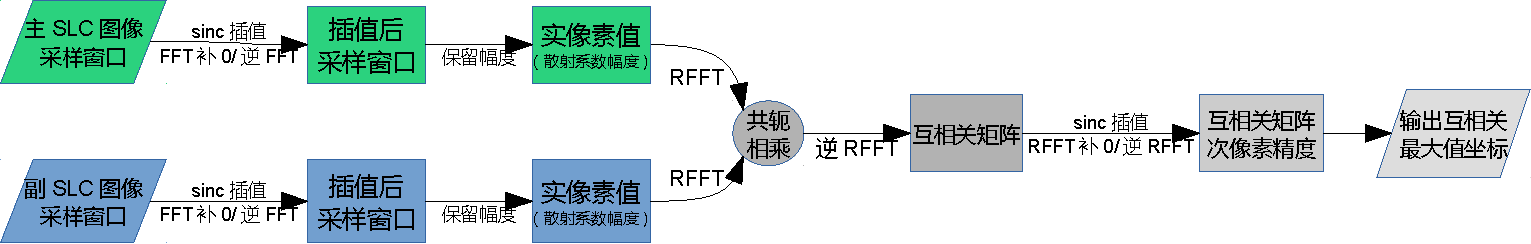
\includegraphics[width=0.99\textwidth]{xcorr2-crop}
\caption{改进的局部配准算法流程}
\note{部分复序列 FFT 算法改成了实序列 FFT 算法(RFFT)}
\label{fig:xcorr2}
\end{figure}

本课题基于上述图像配准算法,设计了并行 SLC 图像配准程序 xcorr2。为了理解 xcorr2 的并行设计,首先要从计算复杂度、内存占用、文件读取三个角度定性分析并行算法的预期性能指标:

\begin{itemize}
    \item \textbf{计算时间}:对于 $64 \times 64 = 4096$ 点的采样窗口,现代桌面 CPU 完成单线程复序列 FFT 计算的时间大约在几 ms 到 50ms 的数量级\cite{fftwbench}。图 \ref{fig:xcorr2} 所示的局部配准需要4次复序列 FFT 或逆 FFT,5次 RFFT 或逆 RFFT,以及一次实复矩阵(逐元素)乘法。以默认参数完成整幅图像配准需要遍历 512 个采样窗口。作为一个简单的估计,完成一次配准需要的 CPU 单线程计算时间约为 10~100s。
    \item \textbf{内存占用}:SAR SLC 图像文件大小可达数GB,但配准过程只需要读取采样窗口的数据。虽然采样窗口默认大小只有 $4096$ 个数据点,但插值后的互相关矩阵可达 $1024^2 = 1M$ 个数据点。考虑到计算过程要存储若干次中间结果,包括 FFT 变换结果、插值序列和互相关矩阵等,将数据点的数量乘以10作为估计值,即需要存储约 10M 个数据点,则可以估计每次局部配准过程需要的内存空间约为数十 MB。并行算法会增加内存开销(正比于计算线程数量),但相对于桌面工作站典型的 4~16GB 的内存配置,预期的内存占用并不大。
    \item \textbf{文件读取延迟}:典型的机械硬盘由于物理延迟则至少在 10ms 的量级\cite{wiki:hddcharacter},相比于 FFT 计算时间仍是不可忽略的。考虑使用单独的线程进行文件读取,并使用更多的内存预存 SLC 数据。
\end{itemize}

\begin{figure}[ht]
\centering
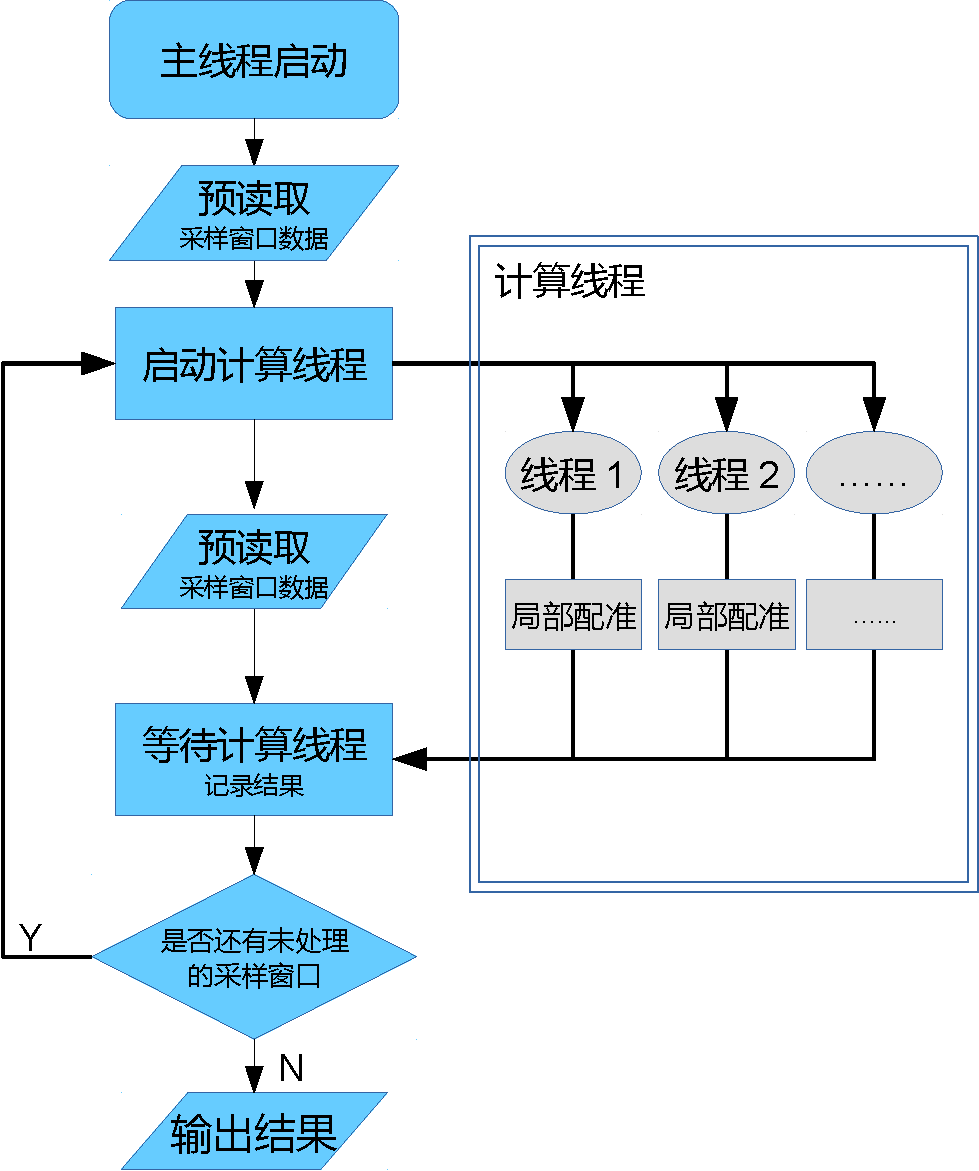
\includegraphics[width=0.6\textwidth]{parallel}
\caption{xcorr2 并行图像配准程序多线程架构(计算线程计算流程同图\ref{fig:xcorr2})} \label{fig:parallel}
\end{figure}

综合上述因素,xcorr2 使用了如图\ref{fig:parallel}所示的主-副多线程并行架构。这一设计的核心是用独立的\textbf{主线程}进行数据预读取,而线程池中的\textbf{计算线程}则负责进行局部配准算法。单线程文件读取可以充分发挥机械硬盘顺序读写的优势,避免多线程磁盘读写(IO)相互竞争影响性能。内存开销方面,主线程每次只提前多读取一组待处理的采样窗口数据,并行内存开销相当于 单线程内存开销 $\times$ 线程数 $\times 2$。

理想情况下,主线程 IO 操作与计算线程局部配准任务完全并行,并且文件读取不慢于一次局部配准所需的时间(按照前面的分析应当是成立的),则并行算法的加速比应当正比于计算线程数量。

\subsection{基于并行规约的图像拼接算法}

图像拼接是 InSAR 数据处理中常见的预处理或后期处理操作。为了得到较大区域的 InSAR 图像,通常可以采用两种图像拼接方法。两种拼接方法的差异仅仅是操作数据的不同,因此本文将合并讨论:

\begin{itemize}
    \item \textbf{SAR 图像帧拼接}:包括 ERS、InSAR 在内的 SAR 卫星,用轨道号(track)和图像帧号(frame)标记不同时间和观测位置的 SAR 数据。同一轨道号的对应的不同图像帧对应的观测区域是在方位向连续的,分成若干帧只是为了便于存储和分发。大地测量应用中,成像范围可能包含多个图像帧,因此要将帧号连续的 SAR 数据文件或者 SLC 图像依次合并,以得到较大的成像区域。GMTSAR 中的 ALOSMerge 程序模块用于进行 ALOS 卫星数据的拼接。
    \item \textbf{InSAR 干涉图拼接}:除了合并 SAR 数据,也可以分区域进行 InSAR 成像再进行图像拼接。因为跨轨道号的 SAR 数据没有成像区域上的连续性,要得到距离向跨多个图像帧的干涉图像,只能在 InSAR 成像后进行拼接。虽然 GMTSAR 没有直接提供拼接程序,但会以 NetCDF 4 文件格式导出相位解缠后的 InSAR 干涉图,该格式可以很方便地使用 Python、Matlab 等编程语言读取和合并。
\end{itemize}

除了 SAR/InSAR 数据处理中的应用,文件拼接也是科研数据处理中常见的操作。数据文件往往受存储器或通信方式的限制,必须分块存储,而在数据处理时要重新合并成连续的数据文件。这类拼接操作的原始数据是串行生成的,其顺序反映了时间或者空间位置上的顺序,因此合并时必须保持特定的拼接的顺序。文件拼接操作 $\oplus$ 满足结合性,但不满足交换性:

\begin{equation}
\begin{split}
    (F_i \oplus F_j) \oplus F_k = F_i \oplus (F_j \oplus F_k) \qquad &\forall F_i, F_j, F_k \in \textrm{\{data files\}} \\
    F_i \oplus F_j \neq F_j \oplus F_i \qquad &\exists F_i, F_j \in \textrm{\{data files\}}
\end{split}
\end{equation}

\begin{figure}[htbp]
\centering
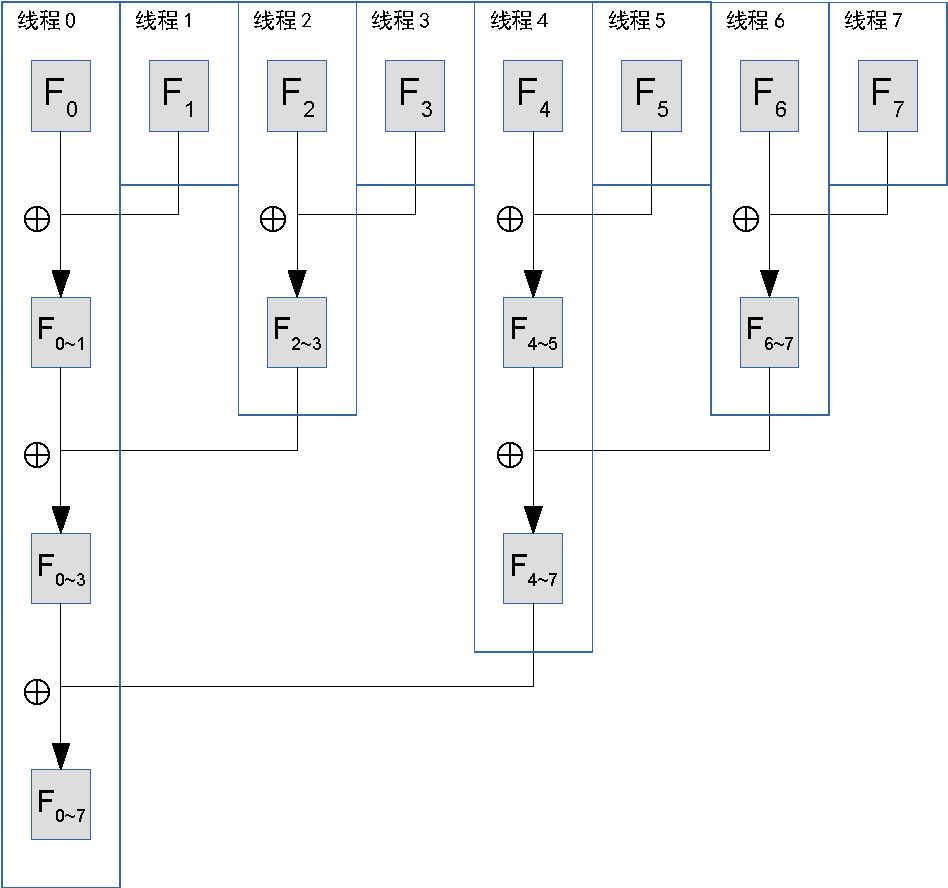
\includegraphics[width=0.65\textwidth]{reduce-crop}
\caption{基于并行规约的图像拼接算法流程示意} \label{fig:reduce}
\end{figure}

文件拼接的顺序要求为程序并行化带来了挑战。这类合并算法,仍可以利用结合性改造为并行算法,这种技术称为并行规约(reduce)。图 \ref{fig:reduce} 展示了并行规约技术的工作流程。规约技术将串行的拼接操作分解为连续的文件序列上的拼接操作,完成一轮拼接后,再通过下一轮迭代将上一轮生成的结果分组拼接,不断迭代直至完成整个文件序列的拼接。并行规约图像拼接算法可以非常简洁地通过程序实现。程序伪代码如图 \ref{fig:reduce-algo} 所示。

\begin{figure}[htbp]
\begin{lstlisting}[language=C]
// threadId: 线程编号
// 全部线程结束后,文件 0 为拼接后的结果
void mergingThread(int threadId) {
    int level = 1;

    while (threadId & level != 0)
        int another = threadId + (1 << level);

        waitThread(another);  // 等待编号为 another 的线程

        // 将编号为 another 的文件合并进编号为 current 的文件
        mergeTwoFile(current, another);
        
        level = level * 2 + 1;
    }

    terminateThread();  // 停止当前线程
}
\end{lstlisting}
\caption{基于并行规约的图像拼接算法伪代码示意}
\label{fig:reduce-algo}
\end{figure}

可以看到,并行规约的图像拼接算法中各工作线程的工作量是不平均的,算法最后会收敛为单线程执行。当要拼接的文件数量较多时可以较好发挥多核心 CPU 的并行计算优势。

理论上,如果忽略文件大小对拼接效率的影响,并且不考虑有效并行线程数的限制,规约技术可以将操作时间从大约 $N \times t$(t 为合并一对文件耗费的时间)缩短至 $\log_2(N) \times t$。

\subsection{其他程序模块的并行优化分析}

InSAR 数据处理是一个复杂计算过程,整个 GMTSAR 软件包含大量 SAR/InSAR 数据处理和辅助分析程序模块。受时间和个人能力所限,本课题无法对整个 GMTSAR 软件进行分析和优化。但值得注意的是,前文所提出的优化方案也应当可以推广到其他程序模块上。本节再通过两个例子说明这一点。

\textbf{干涉图生成模块}(GMTSAR 中的 phasediff 程序)是 InSAR 成像技术的核心,但基本算法并不复杂,只需要简单地计算已经配准的主、副 SLC 图像的相位差、并移除地球曲率造成的相位项即可。对此可以利用与并行图像配准算法同样的思路,将图像分块交给多个线程并行处理。

\textbf{相位解缠模块}(GMTSAR 中的 snaphu 程序)使用 \citet{chen2002phase} 提出的统计耗费网络流算法(Statistical-cost Network-flow algorithm for Phase Unrapping, SNAPHU)进行相位解缠。该算法将解缠相位微分畸变最小化问题转换为最小费用流问题,使用图论中的 Prim 算法和 Dijkstra 算法搜寻相邻的残点\cite{cheng2007insar}。Prim 算法和 Dijkstra 算法的核心均为广度优先搜索,即从单点向相邻的所有点扩展搜索出一个最优结果。广度优先搜索问题一般都可以通过规约技术实现并行。此外,SNAPHU 算法可以对较大的图像进行分片(tile)处理,各分片之间没有数据相关性,因此也可以很方便地以分片为单位并行处理。

此外,多计算任务简单并行也是一种常用的优化手段,即同时运行若干程序实例处理不同的输入数据。虽然这种并行粒度粗,执行小规模计算任务时往往不能实现,但在某些场景下仍可能是最为简单有效的方案。
